\documentclass[article]{jss}\usepackage[]{graphicx}\usepackage[]{color}
% maxwidth is the original width if it is less than linewidth
% otherwise use linewidth (to make sure the graphics do not exceed the margin)
\makeatletter
\def\maxwidth{ %
  \ifdim\Gin@nat@width>\linewidth
    \linewidth
  \else
    \Gin@nat@width
  \fi
}
\makeatother

\definecolor{fgcolor}{rgb}{0.345, 0.345, 0.345}
\newcommand{\hlnum}[1]{\textcolor[rgb]{0.686,0.059,0.569}{#1}}%
\newcommand{\hlstr}[1]{\textcolor[rgb]{0.192,0.494,0.8}{#1}}%
\newcommand{\hlcom}[1]{\textcolor[rgb]{0.678,0.584,0.686}{\textit{#1}}}%
\newcommand{\hlopt}[1]{\textcolor[rgb]{0,0,0}{#1}}%
\newcommand{\hlstd}[1]{\textcolor[rgb]{0.345,0.345,0.345}{#1}}%
\newcommand{\hlkwa}[1]{\textcolor[rgb]{0.161,0.373,0.58}{\textbf{#1}}}%
\newcommand{\hlkwb}[1]{\textcolor[rgb]{0.69,0.353,0.396}{#1}}%
\newcommand{\hlkwc}[1]{\textcolor[rgb]{0.333,0.667,0.333}{#1}}%
\newcommand{\hlkwd}[1]{\textcolor[rgb]{0.737,0.353,0.396}{\textbf{#1}}}%
\let\hlipl\hlkwb

\usepackage{framed}
\makeatletter
\newenvironment{kframe}{%
 \def\at@end@of@kframe{}%
 \ifinner\ifhmode%
  \def\at@end@of@kframe{\end{minipage}}%
  \begin{minipage}{\columnwidth}%
 \fi\fi%
 \def\FrameCommand##1{\hskip\@totalleftmargin \hskip-\fboxsep
 \colorbox{shadecolor}{##1}\hskip-\fboxsep
     % There is no \\@totalrightmargin, so:
     \hskip-\linewidth \hskip-\@totalleftmargin \hskip\columnwidth}%
 \MakeFramed {\advance\hsize-\width
   \@totalleftmargin\z@ \linewidth\hsize
   \@setminipage}}%
 {\par\unskip\endMakeFramed%
 \at@end@of@kframe}
\makeatother

\definecolor{shadecolor}{rgb}{.97, .97, .97}
\definecolor{messagecolor}{rgb}{0, 0, 0}
\definecolor{warningcolor}{rgb}{1, 0, 1}
\definecolor{errorcolor}{rgb}{1, 0, 0}
\newenvironment{knitrout}{}{} % an empty environment to be redefined in TeX

\usepackage{alltt}

%% -- LaTeX packages and custom commands ---------------------------------------

%% recommended packages
\usepackage{thumbpdf,lmodern}
\usepackage{textcomp}
\usepackage[section]{placeins}

%% another package (only for this demo article)
\usepackage{framed}

%% new custom commands
\newcommand{\class}[1]{`\code{#1}'}
\newcommand{\fct}[1]{\code{#1()}}

%% For Sweave-based articles about R packages:
%% need no \usepackage{Sweave}
%% \SweaveOpts{engine=R, eps=FALSE, keep.source = TRUE}



%% -- Article metainformation (author, title, ...) -----------------------------

%% - \author{} with primary affiliation
%% - Separate authors by \And or \AND (in \author).
%% - \AND starts a new line, \And does not.
\author{Harry A. Smith\\Department of Biostatistics and Informatics
\\Colorado School of Public Health\\Skaggs School of Pharmacy\\and
Pharmaceutical Sciences
   \And Laura Saba\\Skaggs School of Pharmacy\\and
Pharmaceutical Sciences}
%% \Plainauthor{Achim Zeileis, Second Author}

%% - \title{} in title case
%% - \Plaintitle{} without LaTeX markup (if any)
%% - \Shorttitle{} with LaTeX markup (if any), used as running title
\title{diffEnrich: An \proglang{R} Package to Compare Functional Enrichment Between Two
Experimentally-derived Groups of Genes by Connecting to the KEGG REST API}
\Plaintitle{diffEnrich: An R Package to Compare Functional Enrichment Between Two
Experimentally-derived Groups of Genes by Connecting to the KEGG REST API}
\Shorttitle{The \proglang{R} Package diffEnrich}

%% - \Abstract{} almost as usual
\Abstract{
  \textbf{Motivation:} To aid in the biological interpretation of a list of candidate
  genes and proteins generated as part of omics studies, researchers quantitate
  the enrichment of known pathways or biological functions among the genes of
  interest. With the advent of new technologies and new experimental designs,
  it is often of interest to compare enrichment of a particular pathway between
  two gene lists (i.e., differential enrichment).
  \textbf{Results:} This package provides a number of functions that are intended to be
  used in a pipeline. Briefly, a function within the package will map
  species-specific ENTREZ gene IDs to their respective Kyoto Encyclopedia of
  Genes and Genomes (KEGG) pathways by accessing the KEGG REST API. The KEGG API
  is used to guarantee the most up-to-date pathway data from KEGG. Next, another
  function will identify significantly enriched pathways in two gene sets
  independently. The user can then identify pathways that are differentially
  enriched between the two gene sets using a third function. This package also
  provides a plotting function.
  \textbf{Availability and implementation:} diffEnrich is freely available on the
  Comprehensive R Archive Network (CRAN). Issues and bug reports can be submitted
  to the GitHub page \url{https://github.com/SabaLab/diffEnrich/issues}.
  \textbf{Supplementary information:} A step-by-step tutorial is provided on the diffEnrich
  GitHub page \url{https://github.com/SabaLab/diffEnrich}, and example data are
  included in the package.

}

%% - \Keywords{} with LaTeX markup, at least one required
%% - \Plainkeywords{} without LaTeX markup (if necessary)
%% - Should be comma-separated and in sentence case.
\Keywords{differential enrichment, KEGG REST API, \proglang{R}}
\Plainkeywords{differential enrichment, KEGG REST API, R}

%% - \Address{} of at least one author
%% - May contain multiple affiliations for each author
%%   (in extra lines, separated by \emph{and}\\).
%% - May contain multiple authors for the same affiliation
%%   (in the same first line, separated by comma).
\Address{
  Laura Saba\\
  University of Colorado\\
  Skaggs School of Pharmacy and Pharmaceutical Sciences\\
  Mail Stop C238\\
  12850 E. Montview Blvd. V20-2124\\
  Aurora, CO 80045\\
  E-mail: \email{Laura.Saba@cuanschutz.edu}
}
\IfFileExists{upquote.sty}{\usepackage{upquote}}{}
\begin{document}


%% -- Introduction -------------------------------------------------------------

%% - In principle "as usual".
%% - But should typically have some discussion of both _software_ and _methods_.
%% - Use \proglang{}, \pkg{}, and \code{} markup throughout the manuscript.
%% - If such markup is in (sub)section titles, a plain text version has to be
%%   added as well.
%% - All software mentioned should be properly \cite-d.
%% - All abbreviations should be introduced.
%% - Unless the expansions of abbreviations are proper names (like "Journal
%%   of Statistical Software" above) they should be in sentence case (like
%%   "generalized linear models" below).

\section[Introduction]{Introduction} \label{sec:intro}

Often high throughput omics studies include a functional enrichment analysis to
glean biological insight from a list of candidate genes, proteins, metabolites,
etc. Functional enrichment examines whether the number of genes in the list
associated with a biological function or particular pathway is more than would
be expected by chance. As an example, enrichment of a particular pathway among
a list of genes that are differentially expressed after an experimental
manipulation may indicate that the pathway has been altered by that
manipulation. This analysis is rather straight forward and many solutions have
been offered (e.g., \cite{HuangDW:2009}; \cite{Kuleshov:2016}; \cite{Liao:2019};
\cite{Subramanian:2005}). A wide variety of databases have also been
used to define these pathways (e.g., \cite{KEGG:2000}) and ontologies
(e.g., \cite{Ashburner:2000}).

One key component of a statistically rigorous functional enrichment analysis is
the definition of a background data set that can be used to estimate the number
of candidate genes that are ``expected'' to be associated with the pathway by
chance, e.g., if 5\% of genes in the background data set are associated with
a pathway then 5\% of candidate gene are expected to be associated with the
pathway by chance. For many study designs, the background data set is
relatively simple to define (e.g., RNA-Seq analyses where the background data
set includes genes expressed above background).

However, for some newer omics technologies, the background data set is hard to
define. For example, LC-MS analysis can be used to identify carbonylated
proteins ( \cite{Petersen:2018}; \cite{Shearn:2019}; \cite{Shearn:2018}).
With this study design, carbonylated proteins are isolated using a BH-derivation
and then LC-MS is used to identify peptides in this isolated sample. The most
appropriate background data set would be proteins present in that tissue, but
this would require a separate analytical analysis. Furthermore, most functional
enrichment analyses involve a single gene list. However, in protein modification
studies, the typical experimental design compares the presence or absence of
particular modified proteins between multiple groups.

When there are two or more gene lists to compare and the background gene list is
not clearly defined, as is often the case in protein modification experiments,
we propose a differential enrichment analysis. In this analysis, we compare the
proportion of genes/proteins from one gene list associated with a particular
pathway to the proportion of genes/proteins from a second gene list that are
associated with that pathway. To easily execute this analysis, we have designed
an R package that uses the KEGG REST API to obtain the most recent version of
the KEGG PATHWAY (\cite{KEGG:2000}) database to initially identify
functional enrichment within a gene list using the entire KEGG transcriptome as
the background data set and then to identify differentially enriched pathways
between two gene lists. This R package includes a function to generate a
``differential enrichment'' graphic.

KEGG is a database resource for understanding high-level functions of a
biological system, such as a cell, an organism and an ecosystem, from genomic
and molecular-level information \url{https://www.kegg.jp/kegg/kegg1a.html}. KEGG is
an integrated database resource consisting of eighteen databases that are
clustered into 4 main categories: 1) systems information (e.g. hierarchies
and maps), 2) genomic information (e.g. genes and proteins), 3) chemical
information (e.g. biochemical reactions), and 4) health information (e.g. human
disease and drugs) \url{https://www.kegg.jp/kegg/kegg1a.html}.


\begin{figure}[!ht]
% \centering
\begin{knitrout}
\definecolor{shadecolor}{rgb}{0.969, 0.969, 0.969}\color{fgcolor}
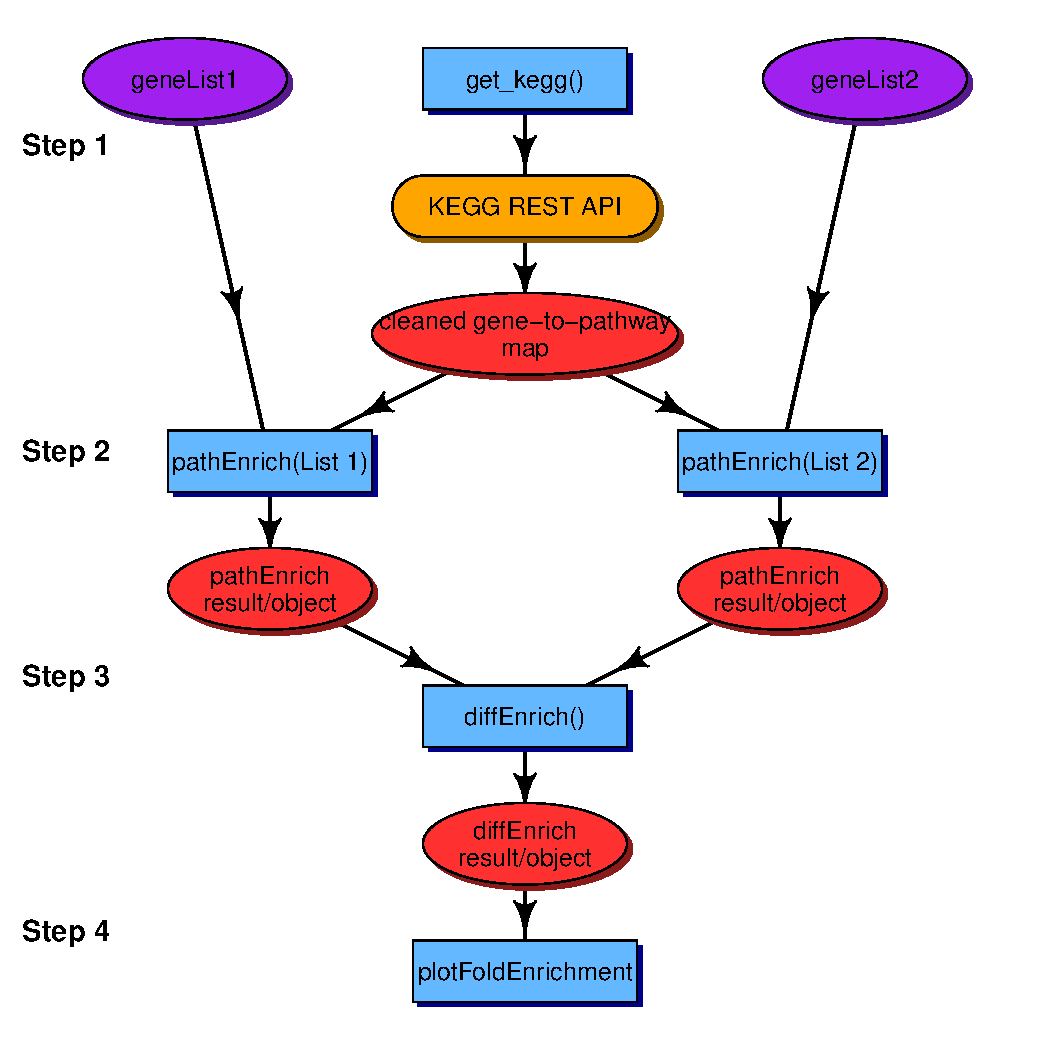
\includegraphics[width=\maxwidth]{figure/visualization-1} 

\end{knitrout}
\caption{\label{fig:flowchart} \textbf{diffEnrich Analysis pipeline.} Functions within
the diffEnrich package are represented by blue rectangles. The data that must be
provided by the user is represented by the purple ovals. Data objects generated
by a function in diffEnrich are represented by red ovals. The external call of
the \code{get\textunderscore kegg} function to the KEGG REST API is represented in yellow.}
\end{figure}

In 2012 KEGG released its first application programming interface (API), and has
been adding features and functionality ever since. There are benefits to using
an API. First, API\textquotesingle s, like KEGG\textquotesingle s, allow users to
perform customized analyses with the most up-to-date versions of the data
contained in the database. In addition, accessing the KEGG API is very easy
using statistical programming tools like R or Python and integrating data
retrieval into user\textquotesingle s code makes the
program reproducible. To further enforce reproducibilty diffEnrich adds a date
and KEGG release tag to all data files it generates from accessing the API. For
update histories and release notes for the KEGG REST API please visit
\url{https://www.kegg.jp/kegg/rest/}.

%% ------------Section 2: Features----------------------------------------------

\section[Features]{Features} \label{sec:feat}

The goal of the diffEnrich package is to compare functional enrichment between
two experimentally-derived groups of genes or proteins. This package provides
four functions that are intended to be used in an ordered pipeline
(Figure~\ref{fig:flowchart}).

\medskip

You can install the released version of diffEnrich from CRAN with:

\begin{knitrout}
\definecolor{shadecolor}{rgb}{0.969, 0.969, 0.969}\color{fgcolor}\begin{kframe}
\begin{alltt}
\hlkwd{install.packages}\hlstd{(}\hlstr{"diffEnrich"}\hlstd{)}
\end{alltt}
\end{kframe}
\end{knitrout}

\subsection{\code{get\textunderscore kegg}: Download and prepare pathways from KEGG API}

First, the \code{get\textunderscore kegg} function is used to connect to the
KEGG REST API and download the data sets required to perform downstream
analysis. Currently, this function supports three species: Homo sapiens, Mus
musculus, and Rattus norvegicus. For a given species, three data sets are
generated: 1) ncbi\textunderscore to\textunderscore kegg: this data set maps NCBI/ENTREZ gene IDs to KEGG gene
IDs, 2) kegg\textunderscore to\textunderscore pathway: this data set maps KEGG gene IDs to their respective
KEGG pathway IDs, and 3) pathway\textunderscore to\textunderscore species: this data set maps KEGG pathway IDs
to their respective pathway descriptions. This function allows the user to save
versioned (based on KEGG release) and time-stamped text files of the three data
sets described above. In addition to these flat files, \code{get\textunderscore kegg} will also create
a named list in R with the three data sets. \code{get\textunderscore kegg} can also read in the saved
text files from a past run and format them for downstream analyses. This
function typically completes in a few seconds, but it is important to note that
the finishing time is dependent on the time it takes to connect to the KEGG API.

The \code{get_kegg} function accesses the KEGG REST API and downloads the data
sets required to perform downstream analysis. This function takes two arguments.
The first, 'species' is required. Currently, diffEnrich supports three species,
and the argument is a character string using the KEGG code: Homo sapiens
(human), use 'hsa'; Mus musculus (mouse), use 'mmu'; and Rattus norvegicus
(rat), use 'rno'. The second, 'path' is also passed as a character string, and
is the path of the directory in which the user would like to write the data sets
downloaded from the KEGG REST API. If the user does not provide a path, the data
sets will be automatically written to the current working directory using the
\code{here::here()} (\cite{kirill:2017}) functionality. These data sets will be
tab delimited files with a name describing the data, and for reproducibility,
the date they were generated and the version of KEGG when the API was accessed.
In addition to these flat files, \code{get_kegg} will also create a named list
in R with the three relevant KEGG data sets. The names of this list will
describe the data set, and are described in Table 1.


\bibliography{refs}


%% -----------------------------------------------------------------------------


\end{document}
